%%**************************************************************
%% Vorlage fuer Bachelorarbeiten (o.ä.) der DHBW
%%
%% Autor: Tobias Dreher, Yves Fischer
%% Datum: 06.07.2011
%%
%% Autor: Michael Gruben
%% Datum: 15.05.2013
%%
%% Autor: Markus Barthel
%% Datum: 22.08.2014
%%**************************************************************

\input{ads/header}
\makeglossaries
%!TEX root = ../dokumentation.tex

%
% vorher in Konsole folgendes aufrufen:
%	makeglossaries makeglossaries dokumentation.acn && makeglossaries dokumentation.glo
%

%
% Glossareintraege --> referenz, name, beschreibung
% Aufruf mit \gls{...}
%
\newglossaryentry{Glossareintrag}{name={Glossareintrag},,description={Ein Glossar beschreibt verschiedenste Dinge in kurzen Worten}}
\newglossaryentry{weight}{name=Weight, description={Gewicht}}


\begin{document}

	% Deckblatt
	\begin{spacing}{1}
		%!TEX root = ../dokumentation.tex

\begin{titlepage}
	\begin{center}
		%{\raisebox{\ht\strutbox-(\totalheight*2)}{\includegraphics[width=50mm,scale=0.5]{images/CLAAS low res.png}}} &
		%%%%%{\raisebox{0cm}{\includegraphics[width=50mm,scale=0.5]{images/CLAAS low res.png}}} &
		\includegraphics[height=2.5cm]{images/dhbw.png}
	\end{center}
	\enlargethispage{20mm}
	\begin{center}
		\vspace*{12mm}	{\LARGE\textbf \titel }\\
		\vspace*{12mm}	{\large\textbf{\arbeit}}\\
		%\vspace*{12mm}	\langdeckblattabschlusshinleitung\\
		%\vspace*{3mm}		{\textbf \abschluss}\\
		\vspace*{12mm}	\langstudiengang{} \studiengang\\
    \vspace*{3mm}		\langanderdh{} \dhbw\\
		\vspace*{12mm}	\langvon\\
		\vspace*{3mm}		{\large\textbf \autor}\\
		\vspace*{12mm}	\datumAbgabe\\
	\end{center}
	\vfill
	\begin{spacing}{1.2}
	\begin{tabbing}
		mmmmmmmmmmmmmmmmmmmmmmmmmm             \= \kill
		\textbf{\langdbbearbeitungszeit}       \>  \zeitraum\\
		\textbf{\langdbmatriknr, \langdbkurs}  \>  \matrikelnr, \kurs\\
		\textbf{\langdbbetreuer}               \>  \betreuer\\
		%\textbf{\langdbgutachter}              \>  \gutachter
	\end{tabbing}
	\end{spacing}
\end{titlepage}

	\end{spacing}
	\newpage

	\pagenumbering{Roman}

	% Sperrvermerk
	%%\input{ads/sperrvermerk}
	%%\newpage

	% Erklärung
	\input{ads/erklaerung}
	\newpage

	% Abstract
	%!TEX root = ../dokumentation.tex

\pagestyle{empty}

\begin{abstract}

A traffic sign detection can nowadays be considered a usual part of automotive vehicles. This is underpinned by the fact that, from the year 2024 on, an EU norm makes such systems mandatory for newly manufactured cars. Traffic sign detection software usually leverages machine learning techniques. Resultingly, images of real traffic signs are necessary for the development of such software. Various datasets exist for this purpose which contain traffic signs from different countries. One property of those datasets is that they can be significantly imbalanced. A reason for this the varying commonness of different traffic sign categories. This can have effects on the quality of detection. One solution is to manually balance those datasets by recording the same number of images for all kinds of traffic signs.

However, for a nearly flawless traffic sign detection, the datasets need to contain different edge cases. Otherwise, future fully autonomous cars can misinterpret traffic signs in specific conditions. One solution is to extend those datasets with real images that are taken in specific weather conditions or where the recognition could be impaired by other factors. This includes vandalism as well as invalid traffic signs. \newline
Another possible solution is to artificially generate such 

A considerable variety of 

An abstract is a brief summary of a research article, thesis, review, conference proceeding or any in-depth analysis of a particular subject or discipline, and is often used to help the reader quickly ascertain the paper's purpose. When used, an abstract always appears at the beginning of a manuscript, acting as the point-of-entry for any given scientific paper or patent application. Abstracting and indexing services for various academic disciplines are aimed at compiling a body of literature for that particular subject.

The terms précis or synopsis are used in some publications to refer to the same thing that other publications might call an ``abstract''. In ``management'' reports, an executive summary usually contains more information (and often more sensitive information) than the abstract does.

Quelle: \url{http://en.wikipedia.org/wiki/Abstract_(summary)}

\end{abstract}
	\newpage %\sqrt{}

	\pagestyle{plain}		% nur Seitenzahlen im Fuß
	
	\RedeclareSectionCommand[beforeskip=\kapitelabstand         ]{chapter} % stellt Abstand vor Kapitelüberschriften ein

	% Inhaltsverzeichnis
	\begin{spacing}{1.1}
		\begingroup
		
			% auskommentieren für Seitenzahlen unter Inhaltsverzeichnis
			\renewcommand*{\chapterpagestyle}{empty}
			\pagestyle{empty}
			
			
			\setcounter{tocdepth}{2}
			%für die Anzeige von Unterkapiteln im Inhaltsverzeichnis
			%\setcounter{tocdepth}{2}
			
			\tableofcontents
			\clearpage
		\endgroup
	\end{spacing}
	\newpage

	% Abkürzungsverzeichnis
	\cleardoublepage
	%!TEX root = ../dokumentation.tex

\addchap{Abkürzungsverzeichnis}
%nur verwendete Akronyme werden letztlich im Abkürzungsverzeichnis des Dokuments angezeigt
%Verwendung: 
%		\ac{Abk.}   --> fügt die Abkürzung ein, beim ersten Aufruf wird zusätzlich automatisch die ausgeschriebene Version davor eingefügt bzw. in einer Fußnote (hierfür muss in header.tex \usepackage[printonlyused,footnote]{acronym} stehen) dargestellt
%		\acs{Abk.}   -->  fügt die Abkürzung ein
%		\acf{Abk.}   --> fügt die Abkürzung UND die Erklärung ein
%		\acl{Abk.}   --> fügt nur die Erklärung ein
%		\acp{Abk.}  --> gibt Plural aus (angefügtes 's'); das zusätzliche 'p' funktioniert auch bei obigen Befehlen
%	siehe auch: http://golatex.de/wiki/%5Cacronym
%	

%%%%%%%%%%%%%%%% IMPORTIERTER CODE %%%%%%%%%%%%%%%%%%%%%%%%%%%%%%%
% provides \AtBeginEnvironment, \patchcmd and \csdef:

\makeatletter
\newcommand{\acroforeign}[1]{}

% patch the environment to print the foreign definition:
\AtBeginEnvironment{acronym}{%
	\def\acroforeign#1{ (#1)}%
}

% patch the acronym definition to safe the foreign definition:
\expandafter\patchcmd\csname AC@\AC@prefix{}@acro\endcsname
{\begingroup}
{\begingroup\def\acroforeign##1{\csdef{ac@#1@foreign}{##1, }}}
{}
{\fail}

% %   renew the first output to include the foreign definition if given:
\renewcommand*{\@acf}[2][\AC@linebreakpenalty]{%
	\ifAC@footnote
	\acsfont{\csname ac@#2@foreign\endcsname\AC@acs{#2}}%
	\footnote{\AC@placelabel{#2}\AC@acl{#2}{}}%
	\else
	\acffont{%
		\AC@placelabel{#2}\AC@acl{#2}%
		\nolinebreak[#1] %
		\acfsfont{(\acsfont{\csname ac@#2@foreign\endcsname\AC@acs{#2}})}%
	}%
	\fi
	\ifAC@starred\else\AC@logged{#2}\fi
}
\makeatother
%%%%%%%%%%%%%%%%%%%%%%%%%% ENDE IMPORTIERTER CODE %%%%%%%%%%%%%%%%%%%%%%

\begin{acronym}[AUTOSAR]
	%\setlength{\itemsep}{-\parsep}
	\acro{CNN}{Convolutional Neural Network}
	\acro{CycleGAN}{Cycle-Consistent Generative Adversarial Network}
	\acro{GAN}{Generative Adversarial Network}
	\acro{GTSRB}{German Traffic Sign Recognition Benchmark}
	\acro{KNN}{Künstliches Neuronales Netz}
	\acro{LSTM}{Long Short-term Memory}
	\acro{PixelRNN}{Pixel Recurrent Neural Network}
\end{acronym}


	% Abbildungsverzeichnis
	\cleardoublepage
	\listoffigures

	% Tabellenverzeichnis
	\cleardoublepage
	\listoftables

	% Quellcodeverzeichnis
	\cleardoublepage
	\lstlistoflistings
	\cleardoublepage

	\pagenumbering{arabic}
	
	\pagestyle{headings}		% Kolumnentitel im Kopf, Seitenzahlen im Fuß

	% Inhalt
	%%%%%\foreach \i in {01,02,03,04,05,06,07,08,09,...,99} {%
	%%%%%	\edef\FileName{content/\i kapitel}%
	%%%%%		\IfFileExists{\FileName}{%
	%%%%%			\input{\FileName}
	%%%%%		}
	%%%%%		{%
	%%%%%			%file does not exist
	%%%%%		}
	%%%%%}

	\chapter{Einleitung}
\section{Problemstellung}
\section{Vorgehensweise}
\section{Ziel der Arbeit}
	\chapter{Stand der Technik}
\section{Momentane Lösungen zur Straßenschilderkennung}

\section{Künstliche Neuronale Netze}
\acused{KNN}
\label{chap:KNNs}
Durch künstliche neuronale Netze (\acsp{KNN}) können Maschinen lernen, bestimmte Probleme zu lösen, ohne dass ein Mensch vorher explizite Regeln dafür definieren muss. Dies steht im Kontrast zur Methode, der Maschine  vorher einen festen, vollständigen Regelsatz bereitzustellen. Letztgenannter Ansatz zeigt in einigen Gebieten nur begrenzten Erfolg, da es für Menschen herausfordernd sein kann, Regelsätze für Vorgänge zu definieren, die unbewusst im Gehirn stattfinden oder viel Kontext erfordern. Zu nennen sind hierbei die visuelle Objekterkennung oder menschliche Sprache. Außerdem können neue, nicht in den Regeln beachtete Situationen dazu führen, dass die Maschine das Problem nicht mehr lösen kann. \cite{DeepLearningBook}

Die Grundidee hinter dem sogenannten \emph{maschinellen Lernen} ist deshalb, dass sich die Maschine selber einen Wissensschatz aufbaut, der ihr beim Lösen des Problems hilft. Dies geschieht, indem die Entwickler ihr reale Trainingsbeispiele zeigen. Möchte man einen Algorithmus trainieren, der Schach spielen soll, kann man ihm beispielsweise eine Vielzahl an realen Schachpartien zeigen. Anhand dessen lernt der Algorithmus verschiedene Strategien und baut ein Spielverständnis auf, das womöglich über die menschlichen Fähigkeiten hinausgeht. \acp{KNN} bauen auf diesem Prinzip auf. Sie implementieren lernbare Funktionen, die eine Abbildung zwischen einer Eingabe und der zugehörigen Ausgabe herstellen. \cite{DeepLearningBook}

In den letzten Jahrzehnten erlebte das maschinelle Lernen und damit auch das Gebiet der \acp{KNN} einen Aufschwung. Es existiert bereits seit Mitte des vergangenen Jarhunderts, wird allerdings erst durch die zunehmende Rechenleistung und die Verfügbarkeit von großen Datenmengen flächendeckend eingesetzt. Einsatzgebiete für \acp{KNN} sind unter anderem die Objekterkennung, das Verstehen von natürlicher Sprache und die Generierung von Text und Bildern. \cite{knnsKompakt}

Die Inspiration für \acp{KNN} bildet die Informationsverarbeitung des Gehirns in Lebewesen. Die kleinste hier betrachtete Einheit ist das Neuron. Neuronen in \acp{KNN} sind konzeptionell inspiriert von realen, biologischen Neuronen, besitzen aber eine abstrahierte Funktionsweise. In \acp{KNN} berechnen sie ein Skalarprodukt ihrer gewichteten Eingangswerte, addieren einen sogennaten \emph{Schwellenwert} (\emph{engl.: Bias}) hinzu und wenden auf das Ergebnis eine nichtlineare Funktion an. Letzere wird auch als Aktivierungsfunktion bezeichnet. 
Diese Aktivierungsfunktion kann analog dazu gesehen werden, dass biologische Neuronen einen Grenzwert (\emph{engl.: threshold}) besitzen, der überschritten werden muss, damit das Neuron \emph{feuert}, also einen Impuls an weitere Neuronen weitergibt. Aktivierungsfunktionen sind notwendig, damit neuronale Netze Probleme lösen können, die über die Fähigkeiten einer linearen Regression hinausgehen. Dadurch können Neuronen eine nichtlineare Abhängigkeit zwischen dem Eingang $x$ und dem Ausgang $y$ umsetzen. \cite{visualApproach}

In Abbildung \ref[fig:neuron] ist ein einzelnes künstliches Neuron eines \acp{KNN} darstellt. Das \emph{Plus-Zeichen} steht für die Berechnung des Skalarprodukts der Eingänge und der darauf addierte Schwellenwert. Die Aktivierungsfunktion wird durch das \emph{Sigmoid}-Zeichen simbolisiert. Der Ausgang (\emph{rechts}) ist das Ergebnis der Berechnung des Neurons. \cite{visualApproach}

\begin{figure}[H]
   \centering
   \includegraphics[width=0.4\textwidth]{images/KNNs/Neuron.png}
   \caption{Einzelnes Neuron eines \acp{KNN} \cite{visualApproach}}
   \label{fig:neuron}
\end{figure}

Um komplexe Probleme lösen zu können, besitzen \ac{KNN} mehrere Neuronen, die miteinander verbunden und in Schichten angeordnet sind. Jede Schicht erhält die Ausgangswerte der vorherigen Schicht als Eingang und gibt die daraus berechneten, neuen Werte an die nächste Schicht weiter. Abbildung \ref{fig:KNN} zeigt ein vollständiges \ac{KNN}. Die Neuronen sind durch Kreise dargestellt und ihre Verbindungen durch Pfeile. \cite{knnsKompakt} 

\begin{figure}[H]
   \centering
   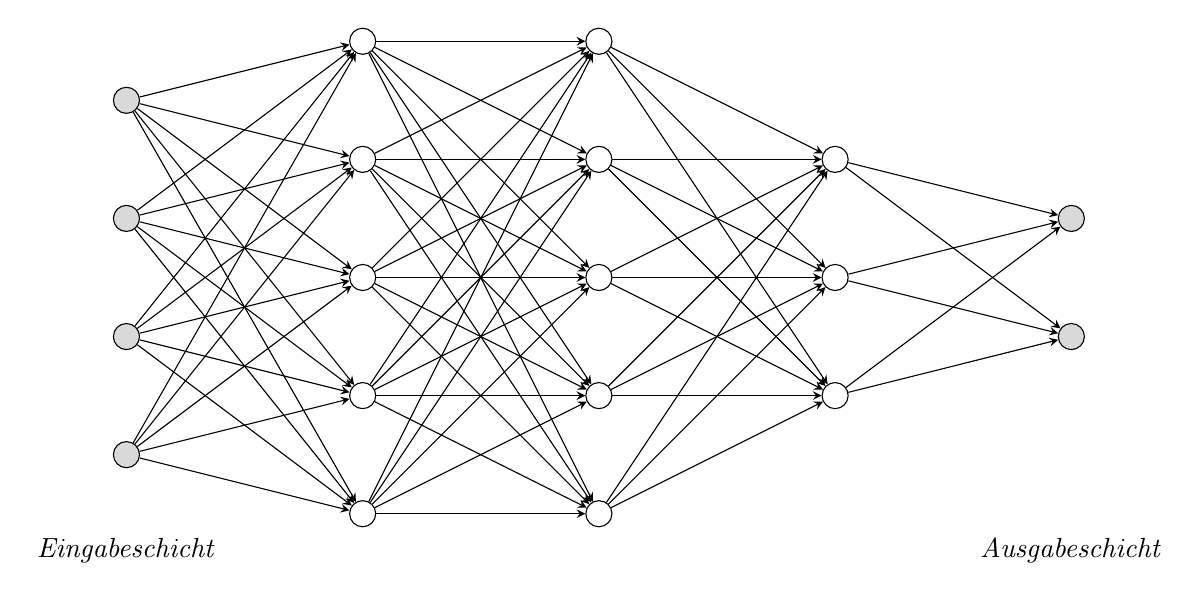
\begin{tikzpicture}[x=1.5cm, y=1.5cm, >=stealth]
      % Input layer
      \foreach \i in {1,...,4}
      \node[circle, draw=black, fill=gray!30] (in-\i) at (0,\i-2) {};
      
      % Hidden layer 1
      \foreach \i in {1,...,5}
      \node[circle, draw=black, fill=white] (h1-\i) at (2,\i-2.5) {};
      
      % Hidden layer 2
      \foreach \i in {1,...,5}
      \node[circle, draw=black, fill=white] (h2-\i) at (4,\i-2.5) {};

      % Hidden layer 3
      \foreach \i in {1,...,3}
      \node[circle, draw=black, fill=white] (h3-\i) at (6, \i-1.5) {};
      
      % Output layer
      \foreach \i in {1,...,2}
      \node[circle, draw=black, fill=gray!30] (out-\i) at (8,\i-1) {};
      
      % Connections
      \foreach \i in {1,...,4}
      \foreach \j in {1,...,5}
      \draw[->] (in-\i) -- (h1-\j);
      
      \foreach \i in {1,...,5}
      \foreach \j in {1,...,5}
      \draw[->] (h1-\i) -- (h2-\j);

      \foreach \i in {1,...,5}
      \foreach \j in {1,...,3}
      \draw[->] (h2-\i) -- (h3-\j);
      
      \foreach \i in {1,...,3}
      \foreach \j in {1,...,2}
      \draw[->] (h3-\i) -- (out-\j);
      
      % Labels
      \node[above] at (0,-2) {\emph{Eingabeschicht}};
      \node[above] at (8,-2) {\emph{Ausgabeschicht}};
      
   \end{tikzpicture}
		\caption{Vollständiges \ac{KNN} \emph{(angelehnt an \cite{visualApproach})}}
      \label{fig:KNN}
\end{figure}

Eine Verbindung stellt dar, dass ein Neuron seinen berechneten Wert an das nachfolgende Neuron weitergibt. Dies geschieht hierbei ausschließlich von \emph{links nach rechts}, womit das \ac{KNN} als \emph{Feedforward-Netzwerk} bezeichnet wird. Die Eingabeschicht erhält die Eingabewerte des Netzwerks, die Ausgabeschicht liefert die Vorhersage des Modells. Zwischen diesen beiden Schichten befinden sich beliebig viele verarbeitende Schichten, die als \emph{Hidden Layer} bezeichnet werden. Die Neuronen der Hidden Layer sind in Abbildung \ref{fig:KNN} in weiß dargestellt. \cite{knnsKompakt}

Die Vorhersage, gekennzeichnet durch die Werte der Ausgabeschicht, hängt von den jeweiligen Parametern der Neuronen des Netzwerks ab. Dies sind die Gewichte (\emph{engl.: weights}) der Verbindungen zwischen den Neuronen sowie der Schwellenwert der Neuronen. Es existieren auch trainierbare Aktivierungsfunktionen, diese sind jedoch vergleichsweise unüblich. Entwickler sind für den Entwurf der Netzwerkarchitektur zuständig, die Parameter werden jedoch durch das Modell trainiert. Zu Beginn besitzt das Modell zufällige Parameter, wodurch es in der Regel nicht die gewünschte Abbildung zwischen Ein- und Ausgabe implementiert. Ein untrainierter Schachalgorithmus spielt demnach augenscheinlich willkürliche Züge. Ein untrainierter Katzenklassifikator besitzt keinen erkennbaren Wissensschatz darüber, welche Charakteristiken eine Katze optisch auszeichnen. Das Ziel des Trainings ist, dass die Parameter des Modells zunehmend gegen das Optimum konvergieren und so das Modell immer plausibler in seinen Vorhersagen wird. \cite{knnsKompakt} \cite{visualApproach}

%---------------------------------------------------------------------------------------------------------------
\subsection{Training}
Das Training von \acp{KNN} benötigt Daten. Zum einen ein Satz an \emph{Trainingsdaten} und zum anderen ein Satz an \emph{Testdaten}. Die Trainingsdaten dienen dazu, das Modell zu verbessern. Eine \emph{Kostenfunktion} berechnet, wie genau die Vorhersagen des Modells auf den Trainingsdaten sind. Darauf basierend wird das Modell optimiert. Die Testdaten dienen zur Messung der Qualität des Modells. Es kann nämlich vorkommen, dass das \ac{KNN} die Trainingsdaten \emph{auswendig} lernt und deshalb hier gute Ergebnisse erzielt, aber eine unzureichende Performanz auf den Testdaten zeigt. Etwa wenn das \ac{KNN} unerwartete Eigenschaften in den Trainingsdaten lernt. Aus diesem Grund werden trainierte Modelle anhand der Testdaten evaluiert. \cite{knnsKompakt}

Die Kostenfunktion bestimmt die durchschnittliche Fehlerrate des \ac{KNN} auf einem gegebenen Datensatz. Sie berechnet somit, gemittelt über alle $m$ Beispiele aus dem Datensatz, die Abweichung des vorhergesagten Wertes $\hat{y}$ von dem tatsächlichen Wert $y$. Für ein einzelnes Beispiel aus dem Datensatz nutzt die Funktion dafür eine \emph{Verlustfunktion} $\mathcal{L}$. Die Verlustfunktion bewertet somit eine einzelne Aussage des \ac{KNN}, während die Kostenfunktion die durchschnittliche Qualität der Aussagen auf dem gesamten Datensatz misst. Folgende Gleichung zeigt die Kostenfunktion: \cite{DeepLearningBook}

\begin{equation}
   \label{eq:costFunctionGeneral}
   J(\theta) = \frac{1}{m} \sum_{i=1}^{m} \mathcal{L}(\hat{y}^{(i)}, y^{(i)})
\end{equation}
Wobei: \newline
\emph{\null\quad\quad $J$: Wert der Kostenfunktion \newline
\null\quad\quad $\theta$: Trainierbare Parameter des Modells \newline
\null\quad\quad $m$: Anzahl der Trainingsbeispiele \newline
\null\quad\quad $i$: Index des momentan betrachteten Trainingsbeispiels \newline
\null\quad\quad $\mathcal{L}$: Verlustfunktion \newline
\null\quad\quad $\hat{y}$: Vorhersage des Modells \newline
\null\quad\quad $y$: Erwarteter Wert}

Die Kostenfunktion $J$ ist abhängig von einem $\theta$. Das $\theta$ ist ein Vektor, der alle Gewichte und Schwellenwerte und damit alle trainierbaren Parameter des \ac{KNN} beinhaltet. Verändern sich die Parameter des \ac{KNN}, dann liefert es andere Aussagen für das $\hat{y}$. Somit ändert sich der Wert der Kostenfunktion, wenn das \ac{KNN} seine Parameter anpasst.  \cite{DeepLearningBook}

Die Gleichung \ref{eq:costFunctionGeneral} kann auch mit dem Operator $\mathbb{E}$ formuliert werden. Er beschreibt den Erwartungswert: \cite{DeepLearningBook}
\begin{equation}
	\label{eq:costFunctionExpectedValue}
	J(\theta) = \mathbb{E}_{x,y}[\mathcal{L}(f(x; \theta), y)]
\end{equation}
Was in Gleichung \ref{eq:costFunctionGeneral} das arithmetische Mittel der Verlustfunktionen ist, wird hier als Erwartungswert der Verlustfunktion geschrieben. Die Fragestellung lautet: \emph{Wenn ein zufälliges Beispiel $x$ und das zugehörige $y$ aus dem Datensatz gezogen werden, was ist dann der erwartete Verlust des Modells?} Die Vorhersage $\hat{y}$ des \ac{KNN} wird hier als $f(x; \theta)$ geschrieben. Dabei ist $f$ das \ac{KNN}, das für ein gezogenes $x$ eine bestimmte Vorhersage trifft. Diese Vorhersage ist zudem abhängig von $\theta$. Diese alternative Darstellung der Kostenfunktion mit dem Operator $\mathbb{E}$ ist relevant für Kapitel \ref{chap:NoGANs}. \cite{DeepLearningBook}

Kostenfunktionen können verschiedene Arten von Verlustfunktionen verwenden. Für diese Arbeit sind sowohl die $\mathcal{L}_1$ und $\mathcal{L}_2$ Verlustfunktionen als auch der \emph{Binary Crossentropy Loss} von besonderer Relevanz.

\paragraph{$\mathcal{L}_1$ Verlustfunktion} Die $\mathcal{L}_1$ Verlustfunktion berechnet für ein gegebenes Beispiel die absolute Abweichung der Vorhersage von dem erwarteten Wert. Sie wird auch als \emph{mittlere absolute Abweichung} \emph{(engl.: mean absolute error)} bezeichnet.
\begin{equation}
   \mathcal{L}_1 = |\hat{y} - y|
\end{equation}

\paragraph{$\mathcal{L}_2$ Verlustfunktion} Die $\mathcal{L}_2$ Verlustfunktion berechnet hingegen die quadratische Abweichung von dem erwarteten Wert. Hier haben somit größe Abweichungen einen stärkeren Einfluss auf den \emph{Verlust} \emph{(eng.: loss)} als bei der $\mathcal{L}_1$ Funktion. Diese Verlustfunktion wird auch als \emph{mittlere quadratische Abweichung} \emph{(engl.: mean squared error)} bezeichnet.
\begin{equation}
   \mathcal{L}_2 = (\hat{y} - y)^2
\end{equation}

\paragraph{Binary Crossentropy Loss} Die Binary Crossentropy Verlustfunktion ist auch als \emph{logarithmische Verlustfunktion} bekannt. Sie eignet sich für binäre Klassifikationen, wo demnach das \ac{KNN} eine Wahrscheinlichkeit zwischen $0$ und $1$ ausgibt. Ein Beispiel hierfür ist, wenn das \ac{KNN} abschätzen soll, ob auf einem Bild eine Katze zu sehen ist oder nicht. Ein Schwellenwert für eine Wahrscheinlichkeit zwischen $0$ und $1$ gibt dann an, ob das Ergebnis als \emph{Ja} oder \emph{Nein} interpretiert wird. Die Binary Crossentropy Verlustfunktion ist in Gleichung \ref{eq:bce-loss} dargestellt. Die Verlustfunktion nutzt die Eigenschaften aus, dass $\log(1) = 0$ ist und der Logarithmus von Werten zwischen $0$ und $1$ negativ ist. Wenn der erwartete Wert $y$ gleich $1$ ist, dann reduziert sich die Verlustfunktion außerdem zu $\mathcal{L} = -\log(\hat{y})$. Entspricht $\hat{y}$ dem erwarteten Wert von $1$, dann ergibt die Verlustfunktion $-\log(1)=0$. Je weiter $\hat{y}$ gegen $0$ strebt, desto größer wird der Wert für $-\log(\hat{y})$. Ist der erwartete Wert $y$ hingegen gleich $0$, dann reduziert sich die Verlustfunktion zu $\mathcal{L} = -\log(1 - \hat{y})$. Hier tritt der umgekehrte Effekt auf. \cite{bce-loss}
\begin{equation}
	\label{eq:bce-loss}
   \mathcal{L}_{BCE} =  - [y \log(\hat{y}) + (1 - y) \log(1 - \hat{y})]
\end{equation}

Das Training des Modells besteht nicht nur daraus, die Vorhersagen des Modells zu bewerten. Damit das Modell in dem nächsten Trainingsdurchlauf idealerweise einen geringeren Wert für die Kostenfunktion erreicht, müssen die trainierbaren Parameter $\theta$ des Modells angepasst werden. Von ihnen hängt der Wert der Kostenfunktion ab. Die Ausgangssituation ist hierbei die folgende: Mit einem gegebenen $\theta$ befindet sich das \ac{KNN} in einem bestimmten Punkt der Kostenfunktion $J(\theta)$. Gesucht ist eine Parameteränderung $\dif\theta$, mit der sich das \ac{KNN} am weitesten an das globale Minimum der Kostenfunktion annähert. Das globale Minimum ist die beste Lösung, die das Modell für die gegebenen Trainingsdaten finden kann und damit das Optimum. Da $J(\theta)$ eine viel-dimensionale Funktion ist, berechnet die Trainingsfunktion diesen Idealwert für $\theta$ nicht numerisch. Stattdessen nähert sich das \ac{KNN} mit jedem Trainingsschritt dem Optimum an. \cite{knnsKompakt}

Nähern tut sich das \ac{KNN} dem Optimum, indem es den Punkt $\theta$ in Richtung des negativen Gradienten der Kostenfunktion bewegt. Also die Richtung, in die, aus der momentanen Ausgangsposition, die Kostenfunktion den steilsten Abstieg besitzt. Pro Trainingsiteration bewegen sich die Parameter $\theta$ nur um einen kleinen Betrag in Richtung des negativen Gradienten. In einem Trainingsschritt kann das \ac{KNN} auf mehrere annotierte Beispiele trainiert werden. Dann bezieht sich die Verlustfunktion $\mathcal{L}$ nicht mehr nur auf ein einzelnes Trainingsbeispiel, sondern auf einen Teil des gesamten Datensatzes. Die Berechnungsformel ist in dem Fall identisch zu den Kostenfunktionen in Gleichungen \ref{eq:costFunctionGeneral} und \ref{eq:costFunctionExpectedValue}. Das ist relevant für Kapitel \ref{chap:GANs}. \cite{knnsKompakt}

Das Training eines \ac{KNN} wird so lange durchgeführt, bis der Gradient einen so geringen Betrag hat, dass sich die Parameter des \ac{KNN} nicht mehr signifikant verändern. Das \ac{KNN} befindet sich hier bestenfalls im globalen Optimum. Der Betrag der Annäherung pro Trainingsschritt ist durch eine sogennante Lernrate $\alpha$ bestimmt. Die Lernrate ist ein \emph{Hyperparameter}, und damit klassischerweise ein nicht-trainierbarer Parameter, da sie durch die Entwickler fest bestimmt wird und nicht durch das Modell selbst gelernt wird. Ist das \ac{KNN} ein mal mit jedem Trainingsbeispiel trainiert worden, spricht man von einer Trainingsepoche \emph{(kurz: Epoche)}. Üblicherweise werden \acp{KNN} über mehrere Epochen trainiert bis die Parameter des Netzes gegen das Optimum konvergieren \cite{knnsKompakt}

\todo[inline]{Auf Ableitung der Kostenfunktion für Berechnung des Gradienten eingehen?}
\todo[inline]{Hier schon Batches erklären und damit darauf eingehen wie mit einer Verlustfunktion über mehrere Trainingsbeispiele trainiert wird}

%---------------------------------------------------------------------------------------------------------------
\subsection{Convolutional Neural Networks}
\acp{KNN} bewähren sich mitunter besonders im Bereich \emph{Computer Vision}. Ein Bereich, der sich mit der Interpretation von Bild- und Videodaten beschäftigt. Hier spielt die Mustererkennung eine tragende Rolle. Es sollen Merkmale erkannt werden, die jedes Objekt eines bestimmten Typs auszeichnen, die jedoch nicht auf jedem Bild die exakt identischen Pixelwerte besitzen. Die typische Form von Katzenohren ist beispielsweise ein Muster, das bei der Katzenerkennung verwendet werden kann. \cite{knnsKompakt}

Verwendet man hierfür jedoch die bisher beschriebene Netzwerkarchitektur, treten verschiedene Probleme auf. Jedes sogenannte \emph{Merkmal} des Eingangs wird über die Eingangsschicht in das \ac{KNN} gespeist. Bei einem Schachalgorithmus kann die Menge aller Merkmale beispielsweise durch die momentane Position aller Figuren auf dem Schachbrett beschrieben werden. Bei der Bildklassifizierung ist jeder Pixel des Bildes ein Merkmal. Ein Netz, das Bilder der Größe 1024x1024 Pixel mit drei Farbkanälen (rot, grün, blau) klassifizieren soll, muss demnach folgende Anzahl an Eingängen verarbeiten: \cite{knnsKompakt}

\begin{equation}
   1024 \cdot 1024 \cdot 3 = 3.145.728
\end{equation}

\acp{KNN}, wie sie bisher gezeigt sind, benötigen dafür eine Architektur mit vielen Neuronen. Das sorgt für mehr trainierbare Parameter und damit unter anderem für eine längere Dauer für das Training sowie für Vorhersagen des Modells. Im Bereich Computer Vision wird deshalb auf eine spezielle Art von neuronalen Netzen namens \ac{CNN} zurückgegriffen, da sie eine effizientere Verarbeitung von solchen Eingabedaten ermöglichen. \cite{knnsKompakt} 

Der Bereich Computer Vision basiert auf der Verarbeitung von Bildern. Ein digitales Bild kann als eine Matrix an Pixelwerten betrachtet werden. Aus diesem Grund ist der Eingang zu einem \ac{CNN} eine Eingangsmatrix. Die Funktionsweise von \acp{CNN} basiert auf der Faltung (engl.: convolution) der Eingangsmatrix mit einer Faltmatrix. Solche Netze besitzen mindestens einen \emph{Convolutional Layer}, der diese Faltung durchführt. Dabei schiebt das \ac{CNN} die Faltmatrix nach und nach über die Eingangsmatrix. Bei jedem Schritt berechnet es dabei das Skalarprodukt der momentan betrachteten Werte der Eingangsmatrix mit den Parametern der Faltmatrix. Das Ergebnis hiervon ist eine neue Matrix. Folgt hierauf eine weitere Schicht, dann erhält sie die Ergebnismatrix der Faltung als Eingabewert und nutzt eine eigene Faltmatrix um erneut eine Faltung durchzuführen. Die trainierbaren Parameter sind dabei die Werte der Faltmatrizen aller Schichten. \cite{DeepLearningBook}

Folgender Algorithmus beschreibt die Funktionsweise einer Faltung: \cite{DeepLearningBook}
\begin{enumerate}
   \item Positioniere die Faltmatrix mittig über einen Pixel der Eingangsmatrix
   \item Berechne das Skalarprodukt aus den Werten der Faltmatrix und den Werten der Eingangsmatrix, die sich unter der Faltmatrix befinden
   \item Schreibe das Ergebnis in eine neue Matrix
   \item Wierholde die Schritte 1-3, bis die Faltmatrix alle Teilmatrizen der Eingangsmatrix abgedeckt hat
\end{enumerate}

Es soll beispielhaft ein Convolutional Layer betrachtet werden. Angenommen, die Eingangsmatrix der Form 7x7 sei ein schwarz-weiß-Bild. Jeder Pixel hat demnach den Wert 0 oder 1. Die Faltmatrix habe die Form 3x3 und zufällig gewählte Parameter. Dann ergibt sich beispielhaft die Faltung, die in Abbildung \ref{fig:convolution} dargestellt ist.

\definecolor{encoder-x}{HTML}{3785D2}
\definecolor{encoder}{HTML}{8BB8E5}
\definecolor{latent}{HTML}{D2D2D2}
\definecolor{decoder}{HTML}{F1A06A}
\definecolor{decoder-x}{HTML}{EC7C32}

\begin{figure}[h]
      \centering
      \includegraphics[width=0.6\textwidth]{images/KNNs/convolution.pdf}
      \caption{Beispiel für eine Faltung eines \ac{CNN} \emph{(angelehnt an \cite{cnn-img})}}
      \label{fig:convolution}
\end{figure}

Zwei Rechenschritte der Faltung sind hier farblich hervorgehoben. Das Skalarprodukt aus dem \color{encoder-x}{blau} \color{black} markierten Teil der Eingangsmatrix und der Faltmatrix ergibt den Wert 4. Die Rechnung hierzu ist:
\begin{equation}
   \color{encoder-x}{1} \color{black}{\cdot 1} + \color{encoder-x}{0} \color{black}{\cdot 0} + \color{encoder-x}{0} \color{black}{\cdot 1} + \color{encoder-x}{1} \color{black}{\cdot 0} + \color{encoder-x}{1} \color{black}{\cdot 1} + \color{encoder-x}{0} \color{black}{\cdot 0} + \color{encoder-x}{1} \color{black}{\cdot 1} + \color{encoder-x}{1} \color{black}{\cdot 0} + \color{encoder-x}{1} \color{black}{\cdot 1} \color{black}{= 4}
\end{equation}
Dieses Ergebnis fügt der Convolutional Layer an den Index (1, 4) der Ergebnismatrix ein. Startet die Faltmatrix in der oberen linken Ecke der Eingangsmatrix und wird nach jedem Rechenschritt um eine Spalte nach rechts verschoben, ist das die vierte Rechnung der Faltung. Das Skalarprodukt der Faltmatrix mit den Werten der \color{decoder-x}{orange}  \color{black} markierten Teilmatrix berechnet der Convolutional Layer dann als letztes. Das Ergebnis ist hier 0, da der betrachtete Teil der Eingangsmatrix überall den Wert 0 besitzt.

In diesem Fall ist das Ergebnis der Faltung eine 5x5-Matrix. Die Größe der Ausgangsmatrix ist abhängig von der Größe der Eingangsmatrix und der Faltmatrix. Eine größere Faltmatrix führt zu einer kleineren Ergebnismatrix, da die Faltmatrix weniger oft über die Eingangsmatrix geschoben werden kann. Auch ist es möglich, dass die Ergebnismatrix die gleichen Dimensionen besitzt wie die Eingangsmatrix oder auch größer ist. Das hängt davon ab, ob die Faltmatrix auch über den Rand der Eingangsmatrix hinausgeschoben wird. \cite{knnsKompakt}

Auch führt ein Convolutional Layer nicht nur eine einzelne Faltung durch, sondern meist mehrere. Jede Faltung hat ihre eigene Faltmatrix und liefert deshalb eine eigene Ergebnismatrix. Jede dieser Faltungen soll ein bestimmtes Merkmal aus dem Eingang erkennen. Beispielsweise kann eine Faltung runde Formen erkennen, während eine andere Faltung gerade Linien erkennt. 

Zusätzlich zu Convolutional Layern besitzen \ac{CNN}-Architekturen sogenannte \emph{Pooling Layer} und \emph{Fully Connected Layer}. Pooling Layer fassen Teile der Eingangsmatrix zu einzelnen Werten zusammen. Beispielsweise existiert das \emph{Max-Pooling}, bei dem der Pooling Layer nur den größten Wert eines Teilbereichs der Eingangsmatrix weitergibt. Die Haupteigenschaft von Pooling Layern ist, dass kleine Schwankungen in den Werten der Eingangsmatrix einen vergleichsweise geringen Einfluss auf die Ausgabe der Schicht haben. Bei Convolutional Layern ist das unter Umständen nicht der Fall, da jeder Wert einen Einfluss auf das jeweilige Skalarprodukt hat. Das ist relevant, da \acp{CNN} generalisieren können sollen, wenn das gesuchte Objekt im Bild leicht unterschiedlich ist. \cite{DeepLearningBook}

Fully Connected Layer sind vergleichbar mit den Schichten eines klassichen \acp{KNN}. Sie bestehen aus Neuronen, die jeweils alle Werte der vorherigen Schicht als Eingang erhalten. \cite{DeepLearningBook}

Abbildung \ref{fig:cnn-architecture} zeigt eine beispielhafte \ac{CNN}-Architektur. 
\begin{figure}[h]
   \centering
   \includegraphics[width=0.8\textwidth]{images/KNNs/cnn-architektur.png}
   \caption{Beispiel für eine \ac{CNN}-Architektur \emph{\cite{cnn-architektur-img}}}
   \label{fig:cnn-architecture}
\end{figure}
Das Netz besitzt abwechselnd Convolutional Layer und Pooling Layer. Das ist üblich für \acp{CNN} \cite{DeepLearningBook}. Auf jede Ergebnismatrix der Faltung führt das \ac{CNN} zudem eine Aktivierungsfunktion aus, die sich \emph{ReLu} \emph{(rectified linear unit)} nennt. Die Schichten sind dazu da, einzelne Merkmale aus dem Eingabebild zu erkennen. Am Ende des \ac{CNN} befindet sich ein Fully Connected Layer, der aus den erkannten Merkmalen eine Vorhersage berechnet. Vorher konvertiert das \ac{CNN} die Ergebnismatrizen in einen einzelnen Vektor, der an den Fully Connected Layer übergeben werden kann. Das ist in der Grafik als \emph{Flatten} bezeichnet. In diesem Beispiel ist das \ac{CNN} ein Klassifikator, der entscheidet, welche Art von Objekt auf dem Bild zu sehen ist.

\section{Bildgenerierung ohne Generative Adversarial Networks}
\subsection{Boltzmann Maschinen}
\subsection{Deep Belief Netzwerke}

\section{Bildgenerierung mit Generative Adversarial Networks}
\acp{GAN} sind eine der eingesetzten Methoden, um Algorithmen zu entwickeln, die neue Daten künstlich generieren können. Dazu zählen zum Beispiel Bilder von Menschen, die zwar realistisch erscheinen, die so aber in der Realität nicht existieren. Die Aufgabe eines \acp{GAN} ist demnach, Daten zu generieren, die denen des definierten Trainingssatzes in einer solchen Weise ähneln, dass nicht mehr unterschieden werden kann, ob ein Bild künstlich generiert ist oder aus dem Trainingssatz stammt. In dem genannten Beispiel besteht der Trainingssatz aus echten Bildern von Menschen, durch die das \ac{GAN} lernt, neue Bilder zu erzeugen. Im weiteren Verlauf wird das Thema \acp{GAN} ausschließlich auf die Bilderzeugung bezogen, auch wenn ebenso andere Anwendungsgebiete existieren. \cite{visualApproach}

Ein \ac{GAN} besteht aus zwei Komponenten. Dem sogenannten \emph{Generator} und dem \emph{Discriminator}. Der Generator erzeugt neue Bilder, während der Discriminator für jedes erzeugte Bild rät, ob es aus dem Trainingssatz stammt, oder ob es künstlich generiert ist. Nur der Discriminator hat dabei Zugriff auf den Trainingsdatensatz. Ihm werden klassischerweise abwechselnd Bilder aus dem Trainingssatz und erzeugte Bilder des Generators gezeigt. Die beiden Komponenten des \acp{GAN} agieren dabei stets gegeinander. Der Generator versucht den Discriminator in die Irre zu führen, dass seine generierten Bilder in Wahrheit aus dem Trainingssatz stammen würden, während der Discriminator versucht, möglichst gut zu erkennen, ob ein Bild echt ist oder nicht. Bei beiden Komponenten handelt es sich dabei um künstliche neuronale Netze \acused{KNN}(\acp{KNN}). \cite{visualApproach}

Während die Bildklassifizierung ein Minimierungsproblem ist, stellt die Bildgenerierung mittels \acp{GAN} ein Min-Max-Problem dar. Bei ersterem wird versucht, die Loss-Function zu minimieren, sodass die Predictions möglichst gut den Labels der Daten entsprechen. Bei \acp{GAN} besteht der Unterschied darin, dass einerseits der Generator die Loss-Function zu minimieren versucht, während andererseits der Discriminator sie zu maximieren versucht.

\begin{equation}
	\min_{G} \max_{D} V(D,G) = E_x[\log(D(x))] + E_z[\log(1-D(G(z)))]
\end{equation}

\subsection{Spieltheorie}
Aus spieltheoreticher Sicht kann das Gegenspiel von Generator und Discriminator auch als \emph{Nullsummenspiel} betrachtet werden.

\subsection{Training}
Zu Beginn sind sowohl der Generator als auch der Discriminator nicht gut geeignet für ihre jeweiligen Aufgaben. Der Generator erzeugt Bilder, die denen des Trainingssatzes nicht änhlich sind, während der Discriminator noch nicht weiß, was die Bilder des Trainingssatzes einzigartig macht. Durch das Training verbessern sich beide Komponenten in ihren Aufgaben. Sie trainieren sich gegenseitig, da sie beide versuchen, das Spiel zu gewinnen.

Das finale Optimum ist, dass der Discriminator so gut in der Unterscheidung zwischen echten und künstlichen Daten wird, wie mit den vorhandenen Daten nur möglich, während der Generator trotzdem in der Lage sein soll, den Discriminator zu überlisten. \cite[S. 656]{visualApproach}

\textbf{Bild ist nicht 100\% korrekt! G wird z.B. nicht trainiert, wenn D richtig lag, aber das Bild aus dem Datensatz stammte.}
\begin{figure}[H]
	\centering
	\includegraphics[width=\linewidth]{../images/GAN-Prozess.drawio.pdf}
	\caption{Trainingsprozess von GANs (angelehnt an \cite[S. 654f.]{visualApproach})}
	\label{fig:gan-trainingsprozess}
\end{figure}

(Auf Emfindlichkeit von GANs für Hyperparameter eingehen)

\subsection{Architekturen}
Die bisher beschriebene Architektur von \acp{GAN} wird auch als \emph{Vanilla \ac{GAN}} bezeichnet. Dies entspricht dem, wie \acp{GAN} in Goodfellows Publikation definiert werden \cite{Goodfellow-GANs}. Forscher und Anwender haben seit dieser Veröffentlichung verschiedene Limitationen und Probleme bei Vanilla \acp{GAN} feststellen können. Insbesondere im Hinblick auf spezielle Einsatzgebiete. Ein hier häufig anzutreffender Begriff ist \emph{Modal Collaps}. Damit ist die Situation gemeint, dass der Generator bei beliebigem Input stets dasselbe Bild generiert. Er lernt, dass ein bestimmtes Bild den Discriminator überlisten kann und generiert es deshalb jedes Mal, egal welchen Input man ihm zuführt. Lösen lässt sich dieses Problem beispielsweise mit sogenannten \acp{CycleGAN}.

\paragraph{CycleGANs}
Ein \ac{CycleGAN} besteht aus zwei miteinander gekoppelten \acp{GAN}. Diese werden klassischerweise als $G$ und $F$ bezeichnet. Bei $G$ handelt es sich um ein Vanilla \ac{GAN}, so wie in diesem Kapitel bisher beschrieben. Erweitert wird das Netzwerk jedoch so, dass es den Output von $G$ an $F$ weitergibt. $F$ erhält somit das von $G$ künstlich generierte Bild als Input. Aufgabe von $F$ ist, daraus den ursprünglichen Input, der $G$ zugeführt wurde, zu reproduzieren. Somit soll das gesamte Netzwerk nicht nur aus einem Input einen gewissen Output generieren können, sondern soll auch von einem gegebenen Output zurück auf den Input schließen können. Dies lässt sich mathematisch so darstellen, dass $G$ und $F$ folgende Abbildungen implementieren:
\begin{equation}
	\mathbf{G}: X\mapsto Y \: \wedge \: \mathbf{F}: Y\mapsto X
\end{equation}
Das Modell $G$ erzeugt somit aus einem gegebenen $X$ ein $Y$, wohingegen $F$ aus dem $Y$ auf das $X$ schließen soll. Die Behebung des Modal Collaps findet dadurch statt, dass das Netzwerk den Output $\tilde{X}$ von $F$ überprüft und diesen mit dem tatsächlichen Input $X$ vergleicht. Es wird überprüft, wie ähnlich sich $\tilde{X}$ und $X$ sind. Liegt eine zu hohe Diskrepanz vor, kann das Netzwerk darauf schließen, dass $G$ Outputs erzeugt, die nicht in direkter Abhängigkeit zu $X$ stehen. 

Was deutlich wird, ist dass hierbei die Idee verworfen werden muss, $G$ ein weißes Rauschen als Input zuzuführen. \acp{CycleGAN} sind für spezielle Anwendungsgebiete gedacht, in denen ausgewählte, und somit nicht-zufällige Eingabebilder verwendet werden. Dazu zählen Gebiete wie \emph{Style Transfer} oder die Transformation von Bildern, respektive Bildelementen. Es wird sich im Verlauf der Arbeit zeigen, dass die Problemstellung dieser Studienarbeit ein solches Anwendungsgebiet darstellt.

\begin{equation}
	L_{GAN}(G, D_Y, X, Y) = E_y[\log{D_Y(y)}] + E_x[\log(1-D_Y(G(x)))]
\end{equation}
\begin{equation}
	L_{cyc}(G, F) = E_x[||F(G(x))-x||_1] + E_y[||G(F(y))-y||_1]
\end{equation}
\begin{equation}
	L(G, F, D_X, D_Y) = L_{GAN}(G, D_Y, X, Y) + L_{GAN}(F, D_X, Y, X) + \lambda L_{cyc}(G, F)
\end{equation}
\cite{cycleGAN}
\paragraph{Wasserstein GANs}

\cite{DeepLearningBook}
\cite{visualApproach}

\section{Vorherige Arbeiten}
\subsection{Generierung deutscher Straßenschilder}
\cite{gtsrbGAN}
\subsection{Generierung taiwanischer Straßenschilder}
\cite{taiwanGAN}

\section{Machine Learning Frameworks}
\subsection{Tensorflow}
\subsection{Pytorch}
\subsection{Weitere}
	\chapter{Konzeption des Modells}
\label{chap:konzept}
\section{Datensatz}
Analog zu der in Kapitel \ref{chap:vorherige-arbeiten-rub} beschriebenen Arbeit wird der \ac{GTSRB} als Datensatz für diese Studienarbeit verwendet. Dies hängt mit der Größe des Datensatzes zusammen, mit der vergleichsweise kleinen Auflösung der einzelnen Bilder und damit, dass sich diese Arbeit auf die Genereriung deutscher Straßenschilder beschränkt. Es soll jedoch in Kapitel \ref{chap:Evaluation} ebenfalls geprüft werden, inwiefern das Resultat der Arbeit genutzt werden kann, um Bilder zu generieren, die Straßenschilder aus anderen Ländern zeigen. Länder, die das Wiener Übereinkommen über Straßenschilder unterzeichnet haben, besitzen vergleichsweise ähnlich aussehende Straßenschilder. Durch das Übereinkommen wird mitunter die grundlegende Form und Farbe verschiedener Schilder bestimmt. \cite{GTSRB} \cite{vienna-convention}

Der \ac{GTSRB} besteht aus mehr als 50.000 Bildern verteilt auf 43 Klassen respektive 43 verschiedenen Arten von Straßenschildern. Beispiele aus dem Datensatz sind in folgender Abbildung dargestellt. \cite{GTSRB}
\begin{figure}[H]
   \centering
   \begin{subfigure}[b]{0.125\textwidth}
       \centering
       \includegraphics[height=\textwidth]{../images/GTSRB/00093.png}
       \caption{}
       \label{fig:gtrsb-paper-bsp-image-1}
   \end{subfigure}
   \hspace{3em}%
   \begin{subfigure}[b]{0.125\textwidth}
       \centering
       \includegraphics[height=\textwidth]{../images/GTSRB/00847.png}
       \caption{}
       \label{fig:gtrsb-paper-bsp-image-2}
   \end{subfigure}
   \hspace{3em}%
   \begin{subfigure}[b]{0.125\textwidth}
       \centering
       \includegraphics[height=\textwidth]{../images/GTSRB/00040.png}
       \caption{}
       \label{fig:gtrsb-paper-bsp-image-3}
   \end{subfigure}
   \hspace{3em}%
   \begin{subfigure}[b]{0.125\textwidth}
    \centering
    \includegraphics[height=\textwidth]{../images/GTSRB/00052.png}
    \caption{}
    \label{fig:gtrsb-paper-bsp-image-4}
\end{subfigure}
      \caption{Beispielbilder aus dem \acs{GTSRB} Datensatz \cite{GTSRB}}
      \label{fig:gtrsb-paper-bsp-images}
\end{figure}

Die Bilder des Datensatzes besitzen unterschiedliche Seitenverhältnisse und verschiedene Auflösungen. Ein Großteil der Bilder ist jedoch kleiner als 100x100 Pixel. Die Bilder basieren auf Videos, die durch die Autoren tagsüber im Straßenverkehr aufgenommen wurden. Die Trainingsbilder sind ungleich auf die Anzahl an Klassen verteilt. Dies hängt mitunter damit zusammen, dass die jeweiligen Schilder nicht gleich häufig im Straßenverkehr verwendet werden. Unterteilt wird der Datensatz in 39.209 Trainingsbilder und 12.630 Testbilder. Da das Ziel dieser Arbeit jedoch nicht ist, einen Klassifikator mit den generierten Bildern zu trainieren, können auch die Testbilder für das Training des Netzes verwendet werden. Es wird nicht zwischen Trainings- und Testbildern unterschieden. \cite{GTSRB}

Der Datensatz wird in dieser Arbeit zunächst so präpariert, dass nur Bilder für das Training verwendet werden, die mindestens 50 Pixel breit oder hoch sind. Dies wird im Verlauf geändert, sodass die Mindestgröße 75 Pixel beträgt.

Die Verteilung der Daten ist auch im präparierten Datensatz nicht homogen. Die nachfolgenden Diagramme zeigen die Verteilung der Daten innerhalb des präparierten Datensatzes. Für die Erhebung mussten die Testdaten manuell ihren Klassen zugeordnet werden.

\definecolor{plotcolor}{HTML}{2b2b2b}

\begin{figure}
\centering
\begin{tikzpicture}
    \begin{axis} [ybar, ylabel={Absolute Häufigkeit}, xlabel={ID des Straßenschilds}, width=\linewidth*0.9, height=\linewidth*0.3, scale only axis=true, xmin=-1, xmax=43, ymin=0, ymax=550, bar width=0.2cm, ytick={0, 100, 200, 300, 400, 500}]
    \addplot[plotcolor, fill] coordinates {
        (0, 40)
        (1, 390) 
        (2, 270) 
        (3, 127)
        (4, 192)
        (5, 113)
        (7, 101)
        (8, 69)
        (11, 396)
        (18, 342)
        (19, 56)
        (20, 31)
        (21, 70)
        (22, 58)
        (23, 144)
        (24, 75)
        (25, 451)
        (26, 118)
        (27, 62)
        (28, 126)
        (29, 60)
        (30, 71)
        (31, 117)
        (6, 14)
        (9, 214)
        (10, 110)
        (12, 424)
        (13, 534)
        (14, 269)
        (15, 77)
        (16, 85)
        (17, 21)
        (32, 12)
        (33, 116)
        (34, 39)
        (35, 121)
        (36, 53)
        (37, 31)
        (38, 195)
        (39, 87)
        (40, 88)
        (41, 19)
        (42, 10)
    };
    \end{axis}
\end{tikzpicture}
\caption{Häufigkeitsverteilung der Arten von Straßenschildern im präparierten Datensatz}
\end{figure}

\begin{figure}
\begin{tikzpicture}
\begin{axis}[ 
xbar, xmin=0, height=\linewidth*0.35, width=\linewidth*0.72,
xlabel={Absolute Häufigkeit},
symbolic y coords={
    Aufhebungen, 
    Einfahrtsverbote,
    Richtungsweiser,
    Vorfahrtsregelungen,
    Geschwindigkeitsbegrenzungen,
    Warnungen,
    },
ytick=data,
nodes near coords, 
nodes near coords align={horizontal},
ytick=data, xmax=2600, xtick={0, 500, 1000, 1500, 2000, 2500}
]
\addplot[plotcolor, fill] coordinates {
    (1227,Vorfahrtsregelungen)
    (1302,Geschwindigkeitsbegrenzungen) 
    (837,Richtungsweiser)
    (55,Aufhebungen)
    (507,Einfahrtsverbote) 
    (2283,Warnungen)};
\end{axis}
\end{tikzpicture} %width=6cm,height=7.59cm
\caption{Häufigkeitsverteilung der Kategorien von Straßenschildern im präparierten Datensatz}
\end{figure}

\section{Framework}
\paragraph{Tensorflow Addons}
\paragraph{Tensorflow Graphics}
Erklären: Wieso benutze ich, wo möglich, Tensorflow Graphics statt OpenCV? Wieso gibt es Tensorflow Graphics überhaupt?
\paragraph{OpenCV}
Erwähnen: OpenCV wird nur da benutzt, wo keine Tensorflow funktionen verwendet werden können. Beeinträchtigt die Performance.

\section{Architektur}
In Kapitel \ref{chap:NoGANs} werden verschiedene generative Netzwerkarchitekturen vorgestellt. Zunächst soll darauf eingegangen werden, welche dieser Herangehensweisen gewählt wird. Jede der Architekturen besitzt ihre Vor- und Nachteile. Der größte Nachteil von \acp{PixelRNN} ist, dass die Pixel eines Bildes nicht parallel zueinander generiert werden können. Dies verlangsamt die Generierung und damit das Training des Modells.

\textbf{Entscheidungsmatrix?}

\section{Datenaugmentation}
Bevor die Piktogramme an den Generator übergeben werden, werden sie zufällig rotiert. Dadurch muss der Generator die Rotation nicht eigenständig lernen und dieser Aspekt der Generierung lässt sich deterministisch bestimmen. Dabei soll die Rotation nicht nur in x-y-Richtung erfolgen, sondern auch eine dreidimensionale Rotation simuliert werden. Und zwar so, als sei das Schild aus einer beliebigen Frontalperspektive aufgenommen worden.

Um bestimmte Transformationen eines Bilds mittels einer Matrixpultiplikation darstellen zu können, wird häufig ein sogenanntes \emph{homogenes Koordinatensystem} verwendet. Dabei wird das Koordinatensystem um eine weitere Dimension erweitert. Ein Punkt $p = [x, y]^\mathsf{T}$ kann somit um einen beliebigen Wert in z-Richtung verschoben werden. Dadurch wird ein Punkt $\tilde{p}$ im homogenen Koordinatensystem durch drei Koordinaten $\tilde{x}$, $\tilde{y}$ und $\tilde{z}$ beschrieben. Transormationen werden in der homogenen Darstellung durchgeführt und anschließend werden daraus die kartesischen Koordinaten $x$ und $y$ bestimmt. Somit erhält man aus der Transformation erneut ein zweidimensionales Bild. \cite{geometric-ops} \cite{math-primer}

Dies wird für eine dreidimensionale Rotation der Piktogramme benötigt. Die Rotation soll durch drei \emph{eulersche Winkel} beschrieben werden. Das bedeutet, dass sie sich aus einer Rotation um die z-Achse, einer um die y-Achse und einer um die x-Achse zusammensetzt. Dies ist in der nachfolgenden Grafik abgebildet. Die bläulichen Balken zeigen dabei die Achse an, um die gedreht wird. Die erste Rotation ist um die z-Achse, wodurch der Balken in die dritte Bildebene geht. \cite{math-primer}

\begin{figure}[H]
	\centering
	\includegraphics[width=0.8\textwidth]{../images/3 Konzeption des Generative Adversarial Networks/Datenaugmentation/Rotation.png}
	\caption{Rotation der Straßenschilder mittels eulerscher Winkel}
	\label{fig:rotation}
\end{figure}

%\begin{figure}[H]
%    \centering
%    \begin{subfigure}[b]{0.2\textwidth}
%        \centering
%        \includegraphics[height=\textwidth]{../images/3 Konzeption des Generative Adversarial Networks/Datenaugmentation/z-axis.png}
%        \caption{Rotation um die z-Achse (\emph{rollen})}
%    \end{subfigure}
%    \hspace{3em}%
%    \begin{subfigure}[b]{0.2\textwidth}
%        \centering
%        \includegraphics[height=\textwidth]{../images/3 Konzeption des Generative Adversarial Networks/Datenaugmentation/y-axis.png}
%        \caption{Rotation um die y-Achse \emph{}}
%    \end{subfigure}
%    \hspace{3em}%
%    \begin{subfigure}[b]{0.2\textwidth}
%        \centering
%        \includegraphics[height=\textwidth]{../images/3 Konzeption des Generative Adversarial Networks/Datenaugmentation/x-axis.png}
%        \caption{Rotation um die x-Achse}
%    \end{subfigure}
%    \caption{Rotationen mittels eulerscher Winkel}
% \end{figure}

Jede Rotation ist durch einen einzelnen Winkel um die jeweilige Achse bestimmt. Kombiniert man die Rotationen, kann die resultierende Tranformation somit durch drei Winkel $(\alpha_z, \alpha_y, \alpha_x)$ eindeutig beschrieben werden. Für die Erzeugung einer zufälligen Rotation müssen randomisierte Werte für diese Winkel bestimmt werden. \cite{math-primer}

Zusätzlich zu der Rotation, soll das Modell die Piktogramme zufällig in ihrer Größe skalieren. Die genannten Augmentationen dienen dazu, die Verteilung der real aufgenommenen Schilder abbilden zu können. Im Datensatz besitzen die Schilder eine unterschiedliche Größe und sind aus verschiedenen Perspektiven aufgenommen. Dadurch dass die Augmentation deterministisch ist, kann sie dazu genutzt werden, um gezielt nur Bilder durch das Modell zu generieren, die aus bestimmten Perspektiven und mit festgelegten Größen generiert wurden. Alternativ kann auch die randomisierte Augmentation beibehalten werden, um eine möglichst große Bandbreite an unterschiedlichen Bildern zu erzeugen.

%Eine Rotation in x- und y-Richtung besitzt folgende sogenannte \emph{Transformationsmatrix} \cite{geometric-ops}:

%\begin{equation}
%    \begin{bmatrix}
%        \cos{\theta} & -\sin{\theta} & 0\\
%        \sin{\theta} & \cos{\theta} & 0\\
%        0 & 0 & 1
%    \end{bmatrix}
%\end{equation}

%Um ein Bild zu Rotieren, multipliziert man in der homogenen Darstellung jeden Pixel des Bilds mit dieser Matrix. Die Winkel $\theta$ sollten alle gleich groß sein, damit das Bild durch die Rotation nicht verzerrt wird. Für die Rotation der Piktogramme der Straßenschilder wird diese Matrix um eine Rotation in z-Richtung erweitert. Die vollständige Gleichung sieht damit wie folgt aus:

%\begin{equation}
%    \begin{bmatrix} \tilde{x} \\ \tilde{y} \\ \tilde{z} \end{bmatrix}
%    =
%    \begin{bmatrix}
%        \cos{\theta_{xy}} & -\sin{\theta_{xy}} & 0\\
%        \sin{\theta_{xy}} & \cos{\theta_{xy}} & 0\\
%        0                 & \sin{\theta_{z}} & 1
%    \end{bmatrix}
%    \cdot \begin{bmatrix} x \\ y \\ 1 \end{bmatrix}
%\end{equation}

%Die linke Seite der Gleichung zeigt $\tilde{p}$, das Ergebnis der Rotation im dreidimensionalen Raum. Die Rotationsmatrix wird dafür mit der homogenen Darstellung des zweidimensionalen Punktes $p$ multipliziert. Die letzte Zeile der Rotationsmatrix stellt die Rotation in z-Richtung dar. Der Term $\sin{\theta_{z}}$ verändert die Pixelwerte in y-Richtung, das heißt das Piktogramm wird in z-Richtung geneigt. Rückblickend wäre jedoch auch eine Rotation in x-Richtung sinnvoll. Dadurch würde der Effekt entstehen, das Foto sei von der Seite aufgenommen worden. Die Rotation der Piktogramme in z-Richtung soll weitaus subtiler sein als in x- und y-Richtung. Deshalb ist $\theta_{z}$ allgemein kleiner als $\theta_{xy}$. \cite{geometric-ops}

%Für die programmatische Implementierung der Rotation mit dem Framework OpenCV muss die Überführung des Bildes aus der homogenen Darstellung zurück in den zweidimensionalen Raum nicht manuell erfolgen. Deshalb soll darauf nicht weiter eingegangen werden. Grundsätzlich wäre dies jedoch der nächste Schritt, um das rotierte Schild in einem zweidimensionalen Bild darstellen zu können.

%\begin{listing}[H]
%    \caption{Rotation der Piktogramme mit OpenCV}
%    \begin{minted}[fontsize=\footnotesize, linenos, breaklines, autogobble]{python}
%        def apply_3d_rotation(img_tensor, theta_xy, theta_z, image_size):
%            """
%            Rotate the img_tensor in x, y and z direction.
%            """
%            transformation_matrix = np.array([
%                [np.cos(theta_xy), -np.sin(theta_xy), 0],
%                [np.sin(theta_xy),  np.cos(theta_xy), 0],
%                [0,                 np.sin(theta_z),  1] 
%            ])
%            rotated_image = cv2.warpPerspective(img_tensor.numpy(), transformation_matrix, (image_size, image_size))
%            return rotated_image
%    \end{minted}
%\end{listing}

%\begin{lstlisting}[language=Python, caption={Rotation der Piktograme mit OpenCV}]
%def apply_3d_rotation(img_tensor, theta_xy, theta_z, image_size):
%    """
%    Rotate the img_tensor in x, y and z direction.
%    """
%    transformation_matrix = np.array([
%    [np.cos(theta_xy), -np.sin(theta_xy), 0],
%    [np.sin(theta_xy),  np.cos(theta_xy), 0],
%    [0,                 np.sin(theta_z),  1] 
%    ])
%    rotated_image = cv2.warpPerspective(img_tensor.numpy(), transformation_matrix, (image_size, image_size))
%    return rotated_image    
%\end{lstlisting}

\section{Training}
Überlicherweise soll beim Training von neuronalen Netzen die Verlustfunktion gegen den Wert \emph{null} streben. Bei diesem Modell soll die Verlustfunktion jedoch gegen einen Wert konvergieren, der größer ist als \emph{null}. In diesem Fall schaffen es weder die Generatoren, die Funktionswerte zu minimieren, noch können die Diskriminatoren die Funktionswerte weiter maximieren. In diesem Fall ist das sogenannte \emph{Nash-Gleichgewicht} erreicht. Das Training ist somit beendet, da sich das Modell mit den gegebenen Daten nicht weiter verbessern kann.
	\chapter{Implementierung und Training}
Viele Trainingsbilder haben nicht das passende Seitenverhältnis. Sie einfach so zu laden würde dazu führen, dass die verzerrt werden. load dataset from directory bietet Parameter an, der dafür sorgt, dass die Bilder gecropppt werden. Central crop, genau das, was ich möchte.

Trainingsbilder die kleiner als 256x256 Pixel sind (was die meisten sind) werden bei der Vergrößerung durch tensorflow vergälttet. Dadurch sind sie nicht verpixelt, sondern nur etwas verschwommen. Gut so.
\section{Hyperparameter}
	\chapter{Augmentation der generierten Bilder}

\label{chap:5}

Wie bereits erwähnt ist das Ziel dieser Studienarbeit nicht alleine die Generierung von Bildern, die Straßenschilder zeigen. Zusätzlich soll die Arbeit einige der in Kapitel \ref{chap:stand-der-technik-strassenschilderkennung} genannten Probleme für die Straßenschilderkennung simulieren. Das Skript \mintinline{python}{generate.py} erlaubt deshalb die Methoden der Augmentierung, die bereits in Tabelle \ref{tab:generate-cli} aufgeführt sind. Diese sind eine \textbf{Bewegungsunschärfe} das Hinzufügen von \textbf{Schnee} und das \textbf{markieren von Schildern als ungültig}. Dafür dient ein Modul \mintinline{python}{utils.image_augmentation}. Für jede der Augmentierungen befinden sich Beispiel-Abbildungen im Anhang.

Die Augmentierung ist weitgehend prozedural implementiert, da keine ausreichend großen Datensätze bekannt sind, die solche Grenzfälle der Straßenschilderkennung zeigen. Diese wären als Trainingsgrundlage für das \ac{CycleGAN} notwendig.

\section{Bewegungsunschärfe}
\label{sec:motion-blur}
Verwackelte Bilder können insbesondere dann entstehen, wenn sich das Fahrzeug mit einer hohen Geschwindigkeit bewegt. Hierbei entsteht eine Bewegungsunschärfe. Dies tritt bei einer Kamera auf, wenn sich das Bild während der Belichtungszeit deutlich verändert. Wenn also die Geschwindigkeit des Fahrzeugs groß ist im Vergleich zur Belichtungszeit. Da sich das fotografierte Objekt zu unterschiedlichen Zeitpunkten an verschiedenen Positionen im Bild befindet, erscheint es als verschwommen. Während bei der Straßenschilderkennung eine Bewegungsunschärfe die Erkennung erschwert, existieren Bereiche, in denen Fotografen absichtlich versuchen sie zu erzeugen. Dazu zählt beispielsweise die Sportfotografie, in der Objekte schneller erscheinen, wenn sie verschwommen zu sehen sind. Die Literatur gibt jedoch Hinweise darauf, dass es nicht trivial sei, die Bewegungsunschärfe mit einer Kamera exakt zu steuern. Beispielsweise wenn die Unschärfe eine bestimmte Intensität haben soll. Aus diesem Grund besteht Interesse daran, Bewegungsunschärfe computergestützt zu erzeugen. \cite{motion-blur}

Ähnlich zu der Funktionsweise von \acp{CNN} basiert die küstliche Erzeugung von Bewegungsunschärfe auf einer Faltung des Bilds mit einer Faltmatrix. Die Idee ist, jeden Pixelwert durch einen Durchschnitt der umliegenden Pixelwerte zu ersetzen. Dabei jedoch linear entlang einer bestimmten Richtung, um eine lineare Bewegung zu simulieren. Je mehr Pixel in die Berechnung des Durchschnitts einbezogen werden, desto stärker erscheint die Bewegungsunschärfe. Die Bewegungsunschärfe in dieser Studienarbeit ist entweder horizontal, vertikal oder diagonal. Es ergeben sich dadurch drei Arten von Faltmatrizen, die in Abbildung \ref{fig:faltmatrizen} gezeigt sind. \cite{motion-blur}

\begin{figure}[h]
	\centering
	\begin{tikzpicture}[baseline=(current bounding box.center)]
		\matrix (A) [nodes={draw, minimum size=9mm}, column sep=-0.2mm] {
			\node{0}; & \node{0}; & \node{0}; \\
			\node{$0.\bar{3}$}; & \node{$0.\bar{3}$}; & \node{$0.\bar{3}$}; \\
			\node{0}; & \node{0}; & \node{0}; \\
		};
		\matrix (B) [nodes={draw, minimum size=9mm}, column sep=-0.2mm, right= of A] {
			\node{0}; & \node{$0.\bar{3}$}; & \node{0}; \\
			\node{0}; & \node{$0.\bar{3}$}; & \node{0}; \\
			\node{0}; & \node{$0.\bar{3}$}; & \node{0}; \\
		};
		\matrix (C) [nodes={draw, minimum size=9mm}, column sep=-0.2mm, right= of B] {
			\node{$0.\bar{3}$}; & \node{0}; & \node{0}; \\
			\node{0}; & \node{$0.\bar{3}$}; & \node{0}; \\
			\node{0}; & \node{0}; & \node{$0.\bar{3}$}; \\
		};
	\end{tikzpicture}
	\caption{Horizontale, vertikale und diagonale Faltmatrix}
	\label{fig:faltmatrizen}
\end{figure}

Die Größe der Faltmatrix gibt die Stärke der Unschärfe an. Bei einer größeren Faltmatrix fließen nämlich mehr Pixel in die Berechnung des Durchschnitts ein. Da die Faltung hier jeden Pixel gleich stark gewichtet, sind alle Parameter der Faltmatrix entlang der simulierten Bewegungsrichtung identisch. Damit jeder Pixel dieselbe Helligkeit besitzt, müssen die Parameter zudem zusammen den Wert \emph{eins} ergeben \cite{motion-blur}. Das ist der Grund, wieso die 3x3-Matrizen in Abbildung \ref{fig:faltmatrizen} die Werte $0.\bar{3}$ haben. Eine 4x4-Matrix hingegen hätte die Werte $0.25$. In dem Modul \mintinline{python}{utils.image_augmentation} existiert die Funktion \mintinline{python}{apply_motion_blur} um auf einen einzelnen Bild-Tensor der Stufe drei eine Bewegungsunschärfe auszuführen. Zusätzlich besitzt die Funktion verschiedene Parameter zur Steuerung der Intensität und der Richtung des Effekts. Listing \ref{code:motion-blur} zeigt, wie die Funktion die Bewegungsunschärfe in diagonaler Richtung durchführt.

\begin{code}
  \begin{minted}{python}
  kernel = np.identity(kernel_size)
  kernel = kernel / kernel_size
  transformed_img = cv2.filter2D(img_tensor.numpy(), -1, kernel)
  \end{minted}
  \caption{\lstinline[language=python]{utils.image_augmentation.py} - Hinzufügen einer diagonalen Bewegungsunschärfe}
  \label{code:motion-blur}
\end{code}

Die Variable \mintinline{python}{kernel} steht für die Faltmatrix. Numpy besitzt eine Funktion \mintinline{python}{identity}, die eine Einheitsmatrix erzeugt. Diese Matrix besitzt auf der Hauptdiagolen Einsen und sonst Nullen. Die \mintinline{python}{kernel_size} gibt die Größe der Matrix an. Damit alle Werte der Matrix summiert den Wert \emph{eins} ergeben, teilt die Funktion die Matrix durch die \mintinline{python}{kernel_size}. In der letzten Codezeile in Listing \ref{code:motion-blur} faltet die Funktion \mintinline{python}{apply_motion_blur} das Eingangsbild mit der Faltmatrix. Dazu nutzt sie die Funktion \mintinline{python}{filter2D} aus der OpenCV Bibliothek. Die Funktion wird genutzt, da sich keine TensorFlow Funktion hat finden lassen, mit der eine derart definierte Faltmatrix auf einem Bild angewendet werden kann, ohne Convolutional Layer zu verwenden. Die Funktion erhält drei Parameter: Den Bild-Tensor, jedoch konvertiert in ein Numpy Array, den Wert $-1$ und die Faltmatrix. Der Wert $-1$ gibt an, dass die Funktion die Anzahl an Farbkanälen des Bilds beibehalten soll.

\section{Ungültige Straßenschilder}
In Kapitel \ref{chap:stand-der-technik-strassenschilderkennung} ist bereits beschrieben, dass als ungültig markierte Schilder eine Herausforderung für heutige Straßenschilderkennungen darstellen können. Aus diesem Grund implementiert diese Studienarbeit den Anwendungsfall. Ungültige Schilder sind im Straßenverkehr meist durch ein orangefarbenes Kreuz gekennzeichnet.

Bei der Umsetzung bieten sich verschiedene Möglichkeiten. Zum einen kann das \ac{CycleGAN} darauf trainiert werden, solche Bilder eigenständig zu generieren. Dafür benötigt das Modell Trainingsdaten mit ungültigen Schildern. Der Datensatz müsste somit um reale Bilder ergänzt werden, was nicht ohne weiteres möglich ist. Es wäre jedoch auch denkbar, bereits vorhandene Trainingsbilder mit einer Bildbearbeitungssoftware so anzupassen, dass sie ungültige Schilder zeigen.

Eine weitere Möglichkeit ist, das Kreuz, das die Ungültigkeit eines Schilds markiert, nachträglich in die generierten Bilder des \ac{CycleGAN} einzufügen. Die Besonderheit ist hierbei, dass die Straßenschilder zufällig rotiert und skaliert sind. Die Augmentierungsfunktion muss das Kreuz vorher so transformieren, dass es sich stets zentral und mit einer angepassten Rotation auf dem Schild befindet. Da hierfür keine zusätzlichen Trainingsdaten nötig sind, implementiert das Modul  \mintinline{python}{utils.image_augmentation} dieses Vorgehen. Die Funktion dafür heißt \mintinline{python}{make_street_sign_invalid}. 

Für zukünftige Arbeiten ist ein weiterer Ansatz, die Kreuze vor der Bild-zu-Bild Generierung auf die Piktogramme einzufügen. Dafür können Entwickelnde die Funktion \mintinline{python}{make_street_sign_invalid} verwenden. Sie müssen das entstehende Bild anschließend skalieren und rotieren und an das \ac{CycleGAN} als Eingangsdomäne $X$ übergeben. Auch hierfür benötigt das Modell zusätzliche Trainingsdaten. Es muss jedoch nicht von alleine lernen, das Kreuz zu erzeugen, da dies bereits im Eingangsbild enhalten ist. Außerdem kann der Quellcode genutzt werden, um andere Objekte auf die Schilder einzufügen. Beispielsweise wenn Entwickelnde das \ac{CycleGAN} erweitern wollen, um Vandalismus auf Straßenschildern zu simulieren.

In dem Ordner \mintinline{python}{Augmentation} unter \href{https://drive.google.com/drive/u/1/folders/1310Eb5WDgaszu47k6V8St5m-QtQV1Ocg}{\textbf{dem Link des Datensatzes}} (Stand: 09.06.2023) befindet sich das rohe Bild eines orangefarbenen Kreuzes auf einem transparenten Hintergrund. Abbildung \ref{fig:cross} zeigt dieses Bild.
\begin{figure}[h]
	\centering
	\includegraphics[width=0.15\textwidth]{images/augmented images/cross.png}
	\caption{Kreuz auf transparentem Hintergrund, das Schilder als ungültig kennzeichnet}
	\label{fig:cross}
\end{figure} 
Prinzipiell implementiert die Funktion \mintinline{python}{make_street_sign_invalid} folgendes: Sie augmentiert das Bild genau wie das übergebene Straßenschild und fügt es dann auf das Schild ein. Aufrufende Funktionen müssen deshalb nicht nur ein generiertes Schild übergeben, sondern auch den Wert für die Skalierung sowie die Transformationsmatrix, die zu diesem generierten Bild geführt hat. Die Funktion \mintinline{python}{make_street_sign_invalid} kann das Kreuz dann mit den gleichen Parametern skalieren und rotieren wie das Straßenschild. Dadurch fügt die Funktion das Kreuz zentriert auf das Straßenschild ein. Die Funktion \mintinline{python}{make_street_sign_invalid} besteht in verkürzter Form aus dem Code in Listing \ref{code:invalid-sign}.

\begin{code}
	\begin{minted}{python}
cross = preprocess_image.transform_image(cross, content_size, transformation_matrix, bg_is_white=False)
img_tensor = tf.concat([img_tensor, tf.ones_like(img_tensor[:, :, 0:1])], axis=-1)
# img_tensor and cross are numpy arrays here
img_tensor.paste(cross, (0, 0), cross)
	\end{minted}
	\caption{\lstinline[language=python]{utils.image_augmentation.py} - Schilder als ungültig markieren}
	\label{code:invalid-sign}
\end{code}

Die Variable \mintinline{python}{cross} ist ein Bild-Tensor der Stufe drei, der das Kreuz enthält. Dabei hat der Tensor jedoch nicht wie in dieser Studienarbeit üblich die Form \emph{(256, 256, 3)} sondern \emph{(256, 256, 4)}. Das liegt daran, dass jeder der $256\cdot 256$ Pixel zusätzlich zu den Werten für rot, grün und blau auch einen \emph{Alphakanal} besitzt. Dieser gibt an, wie transparent der Pixel ist. Der Wert $0$ bedeutet, dass der Pixel vollständig transparent ist, während der Wert $1$ bedeutet, dass der Pixel vollständig deckend ist. Der transparente Hintergrund um das Kreuz besitzt damit überall einen Alpha-Wert von $0$. In der ersten Codezeile in Listing \ref{code:invalid-sign} wird das Bild des Kreuzes augmentiert. Dazu wird die gleiche Funktion genutzt wie für die Datenaugmentierung des \ac{CycleGAN}: \mintinline{python}{transform_image} aus \mintinline{python}{utils.preprocess_image}. Neben dem Tensor \mintinline{python}{cross} übergibt die Funktion hier die beiden Transformationsgrößen sowie den Parameter \mintinline{python}{bg_is_white=False}. Damit füllt die Funktion \mintinline{python}{tranform_image} den Hintergrund des Bilds mit vollständig transparenten statt mit weißen Pixeln auf.

In einem nächsten Schritt fügt die Funktion dem generierten Eingangsbild \mintinline{python}{img_tensor} einen Alphakanal mit den Werten $1$ hinzu. Dafür existiert die Funktion \mintinline{python}{tf.concat}, die mehrere Tensoren zusammenfügen kann. Einer ihrer Parameter ist eine Liste von Tensoren, die miteinander konkateniert werden sollen. Der erste Tensor ist der Eingangstensor der Form \emph{(256, 256, 3)}. Der zweite Tensor hat die Form \emph{(256, 256, 1)} und enthält nur Einsen als Werte. Der Code \mintinline{python}{img_tensor[:, :, 0:1]} entnimmt aus dem Eingangsbild einen einzelnen Farbkanal, während die Funktion \mintinline{python}{tf.ones_like} diesen Farbkanal komplett mit Einsen auffüllt. Der Parameter \mintinline{python}{axis=-1} legt fest, dass der neu erzeugte Alphakanal an die letzte Achse des Tensors angefügt wird, an der sich die Farbkanäle befinden. Der so erzeugte Tensor hat die Form \emph{(256, 256, 4)} und enthält neben den Farbwerten auch einen Alphakanal.

Das Bild wird dadurch nicht verändert, da beide Bilder nun die gleiche Anzahl an Farbkanälen haben, kann die Funtkion \mintinline{python}{make_street_sign_invalid} das Kreuz jedoch nun auf das Eingangsbild einfügen. Dazu dient die Funktion \mintinline{python}{paste} aus der Bibliothek Pillow. Sie fügt das Kreuz an die Koordinaten $(0,0)$ ein. Der dritte Parameter mit dem Wert \mintinline{python}{cross} sorgt dafür, dass die transparenten Pixel des Kreuzes erhalten bleiben und damit das Eingangsbild nicht überdecken. Vor der Anwendung der Pillow-Funktion werden die Bilder in Numpy Arrays konvertiert. \cite{pillow}

\section{Schnee}

Schnee ist eine Wetterbedingung, die, ausgehend von Kapitel \ref{chap:stand-der-technik-strassenschilderkennung}, eine Auswirkung auf die Straßenschilderkennung haben kann. Es ließen sich keine Veröffentlichungen finden, die das künstliche Einfügen von Schnee auf Bilder in eine in diesem Rahmen umsetzbare Art und Weise aufzeigen. Aus diesem Grund basiert die Implementierung auf folgendem Vorgehen: Ein Bildbearbeitungsprogramm wurde genutzt, um ein Bild aus künstlichem Schnee zu erstellen. Anschließend daran wurde das Vorgehen in dem Bildbearbeitungsprogramm als ein Algorithmus formuliert, der das Vorgehen in Python automatisieren kann.

Der Algorithmus besteht aus folgenden Schritten:
\begin{enumerate}
  \item Erstelle ein Bild, das aus zufälligen schwarzen und weißen Pixeln besteht. Die Anzahl an weißen Pixel soll kleiner sein als die der schwarzen Pixel.
  \item Führe auf dem Bild ein Gaußsches Weichzeichen aus. Hierdurch verschmieren die einzelnen weißen Pixel zu größeren Punkten.
  \item Führe auf dem Bild eine Bewegungsunschärfe aus. Dadurch wird die Bewegung der Schneeflocken entlang einer Windrichtung simuliert.
  \item Mache den schwarzen Hintergrund transparent und füge das erstellte Bild auf ein generiertes Straßenschild-Bild ein.
\end{enumerate}

Die Funktion \mintinline{python}{add_snow} implementiert diesen Algorithmus. Sie erzeugt die zufälligen schwarzen und weißen Pixel mittels einer Binomialverteilung. Für jeden Pixel existieren zwei Mögliche \emph{Ziehungen} aus der Verteilung: Schwarz (0) oder weiß (1). Ein $p$ gibt an, wie hoch die Wahrscheinlichkeit dafür ist, dass ein weißer Pixel gezogen wird. Die Problemstellung lässt sich für jeden Pixel als ein Zufallsexperiment mit zwei möglichen Ausgängen beschreiben. Das ist der Grund, wieso die Funktion hier eine Binomialverteilung implementiert. Dafür bietet TensorFlow die Funktion \mintinline{python}{tf.random.stateless_binomial}. Das auf dem Bild ausgeführte gaußsche Weichzeichen sorgt dafür, dass jeder Pixel \emph{verschwommen} wird. Das kann mit dem vorgehen für die Bewegungsunschärfe verglichen werden. Mit dem Unterschied, dass die Unschärfe hier nicht linear in eine Richtung zeigt, sondern kreisförmig um jeden Pixel ist. Damit wird aus jedem weißen Pixel ein kreisförmiger Punkt, der eine Schneeflocke darstellen soll. Für das gaußsche Weichzeichen bietet die Bilbiothek TensorFlow Addons die Funktion \mintinline{python}{tfa.image.gaussian_filter2d}. Für die anschließende Bewegungsunschärfe ruft die Funktion \mintinline{python}{add_snow} die in Abschnitt \ref{sec:motion-blur} beschriebene Funktion \mintinline{python}{add_motion_blur} auf. \cite{geometric-ops}

Diese Augmentierung der Bilder ist zusätzlich für eine weitere Fragestellung genutzt: \textbf{\emph{Kann das \ac{CycleGAN} lernen, verschneite Bilder eigenständig zu generieren?}}. Dazu existiert eine \emph{Checkpoint}-Datei, die Parameter des U-Net-Modells enthält, wenn es auf verschneiten Bildern trainiert ist. In dem \href{https://drive.google.com/drive/folders/1310Eb5WDgaszu47k6V8St5m-QtQV1Ocg?usp=sharing}{\textbf{Link des Datensatzes}} befinden sich die Trainingsbilder unter dem Pfad \mintinline{python}{'Train with Snow'}.

Die Basis für das Training stellt das für 200 Epochen trainierte U-Net-basierte \ac{CycleGAN} da. Auf den verschneiten Bildern ist das Modell zusätzliche 20 Epochen trainiert. Abbildung \ref{fig:snow-imgs-training} zeigt den Verlauf des Trainings. Die Bilder stammen aus verschiedenen Trainingsepochen, wobei das erste Bild zu der ersten Epoche korrespondiert und das letzte Bild zu der zwangigsten Epoche.

\begin{figure}[H]
	\centering
  \captionsetup[subfigure]{labelformat=empty}
	\begin{subfigure}[b]{0.125\textwidth}
		 \centering
		 \includegraphics[height=\textwidth]{../images/snow generation/training/1.png}
	\end{subfigure}
	\hspace{0.5em}%
	\begin{subfigure}[b]{0.125\textwidth}
		 \centering
		 \includegraphics[height=\textwidth]{../images/snow generation/training/2.png}
	\end{subfigure}
	\hspace{0.5em}%
	\begin{subfigure}[b]{0.125\textwidth}
		 \centering
		 \includegraphics[height=\textwidth]{../images/snow generation/training/6.png}
	\end{subfigure}
	\hspace{0.5em}%
	\begin{subfigure}[b]{0.125\textwidth}
	 \centering
	 \includegraphics[height=\textwidth]{../images/snow generation/training/8.png}
  \end{subfigure}
  \hspace{0.5em}%
  \begin{subfigure}[b]{0.125\textwidth}
	\centering
	\includegraphics[height=\textwidth]{../images/snow generation/training/11.png}
	\end{subfigure}
	\hspace{0.5em}%
	\begin{subfigure}[b]{0.125\textwidth}
		\centering
		\includegraphics[height=\textwidth]{../images/snow generation/training/12.png}
	\end{subfigure}
	\hspace{0.5em}%
	\begin{subfigure}[b]{0.125\textwidth}
		\centering
		\includegraphics[height=\textwidth]{../images/snow generation/training/18.png}
	\end{subfigure}
 \caption{Trainingsverlauf des \ac{CycleGAN} um Bilder mit Schnee zu erzeugen}
 \label{fig:snow-imgs-training}
 \end{figure}

Abbildung \ref{fig:snow-imgs-unet} zeigt Bilder, die das Modell am Ende des Trainings erzeugt. Es zeigt sich, dass das \ac{CycleGAN} eigenständig verschneite Bilder generieren kann. 20 Epochen werden hier als eine akzeptable Dauer für ein zusätzliches Training betrachtet. Ausgehend davon können Anwendende die vortrainierten Modelle dieser Studienarbeit nutzen, um es auf eigene Augmentation zu trainieren. Ebenso kann erprobt werden, inwiefern das \ac{CycleGAN} lernen kann, Bewegungsunschärfe und ungültige Schilder zu erzeugen.
 
 \begin{figure}[H]
	\centering
  \captionsetup[subfigure]{labelformat=empty}
	\begin{subfigure}[b]{0.15\textwidth}
		 \centering
		 \includegraphics[height=\textwidth]{../images/snow generation/1.png}
	\end{subfigure}
	\hspace{1em}%
	\begin{subfigure}[b]{0.15\textwidth}
		 \centering
		 \includegraphics[height=\textwidth]{../images/snow generation/2.png}
	\end{subfigure}
	\hspace{1em}%
	\begin{subfigure}[b]{0.15\textwidth}
		 \centering
		 \includegraphics[height=\textwidth]{../images/snow generation/3.png}
	\end{subfigure}
	\hspace{1em}%
	\begin{subfigure}[b]{0.15\textwidth}
	 \centering
	 \includegraphics[height=\textwidth]{../images/snow generation/4.png}
	\end{subfigure}
	 \hspace{1em}%
	\begin{subfigure}[b]{0.15\textwidth}
	 \centering
	 \includegraphics[height=\textwidth]{../images/snow generation/5.png}
  \end{subfigure}
 \caption{Generierte Bilder des \ac{CycleGAN} mit Schnee}
 \label{fig:snow-imgs-unet}
 \end{figure}

 Abbildung \ref{fig:snow-imgs-generated} im Anhang zeigt weitere verschneite Bilder, die durch das \ac{CycleGAN} generiert sind.
	\chapter{Das finale Produkt}
\section{Benchmark}
	\chapter{Zusammenfassung}

Diese Arbeit befasst sich mit der künstlichen Erzeugung von Bildern, die Straßenschilder zeigen. Zusätzlich ist eine Augmentierung der generierten Bilder auf Grenzfälle der Straßenschilderkennung implementiert.

Wie bereits eine vorherige Arbeit gezeigt hat, ist die Generierung solcher Bilder mit \acp{CycleGAN} möglich. In dieser Arbeit erzielt ein U-Net-basiertes \ac{CycleGAN} dabei bessere Ergebnisse und ist schneller zu trainieren. Allgemein zeigt sich anhand der Evaluation, dass sich die erzeugten Datensätze von realen Trainingsdaten unterscheiden. Trotzdem können sie einen Klassifikator verbessern, indem sie als \textbf{zusätzliche} Trainingsdaten genutzt werden. Das deutet darauf hin, dass sie sich als zusätzliche Trainingsdaten eignen. Verschiedene Möglichkeiten der Verbesserung existieren dennoch.

Diese Arbeit zeigt, dass \acp{CycleGAN} ebenso lernen können, bestimmte Augmentierungen für die Straßenschilderkennung eigenständig zu lernen. So etwa das Generieren von Bildern mit Schnee. Dabei sind in dieser Arbeit in etwa 20 zusätzliche Trainingsepochen nötig. Auf dem verwendeten System der \ac{DHBW} entspricht das einer Trainingsdauer des U-Net-basierten Modells von etwa $1,7$ Stunden.

Die prozedural erzeugten Augmentierungen von Bewegungsunschärfe, ungültigen Schildern und Schnee verringern zudem die Genaugkeit eines Klassifikators für die Straßenschilderkennung. Das gibt Hinweise darauf, dass solche Bilder Datensätze für die Straßenschilderkennung erweitern können.

Zusammenfassend lässt sich demnach sagen, dass die Arbeit einige der festgelegten Ziele erfüllt. Jedoch sind die generierten Bilder nicht vollständig fotorealistisch. Das gilt auch für die Augmentierungen.

Zukünftige Arbeiten können hier anknüpfen, um inbesondere weitere Grenzfälle der Straßenschilderkennung zu simulieren. Auch um die momentanen Augmentierungen realistischer zu gestalten. Weitere Arbeiten auf dem Gebiet können sich zudem damit beschäftigen, Bilder für die Straßenschilderkennung zu erzeugen, die eine größere Menge an Hintergrund um die Schilder zeigen. Insbesondere um Grenzfälle der Straßenschilderkennung weiter zu simulieren. Auch ist denkbar, Videosequenzen künstlich zu generieren.

	\clearpage

	% Literaturverzeichnis
	\cleardoublepage
	\printbibliography

	% Glossar
	\printglossary[style=altlist,title=\langglossar]
	
	%% BILDER IM ANHANG NICHT IN ABBILDUNGSVERZEICHNIS AUFLISTEN
	\let\svaddcontentsline\addcontentsline
	\renewcommand\addcontentsline[3]{%
		\ifthenelse{\equal{#1}{lof}}{}%
		{\ifthenelse{\equal{#1}{lot}}{}{\svaddcontentsline{#1}{#2}{#3}}}}
	
	% sonstiger Anhang
	\clearpage
	\appendix
	% !TeX root = ../dokumentation.tex

\addchap{\langanhang}

%(Beispielhafter Anhang)
 

{\Large
\begin{enumerate}[label=\Alph*.]
	\item test
	\item test
	\item test
\end{enumerate}
}
\pagebreak
	
\end{document}
